\chapter{상태, 측정, 복소 벡터 공간}

\lectureoverview{양자역학은 상태가 무엇을 뜻하는지 바꾸는 데서 시작한다. 먼저 상태와 결정론적 갱신이라는 고전적 유형을 분리해 살펴본 다음, 결과가 두 가지인 스핀 실험으로 그 유형이 성립하지 않음을 드러낸다. 이에 대한 수학적 대응은 쌍대벡터, 내적, 노름, 직교성을 갖춘 복소 벡터 공간이다.}

\section{고전적 유형: 상태와 갱신}

일단 다른 모든 것과 분리된 닫힌 계에서 시작하자. 여기서 \emph{계}라는 말은 원초적 개념이다. 예측하고자 하는 이력을 지닌 대상을 뜻한다. \emph{상태}란 그 예측을 하려면 한 시점에 알아야 하는 모든 것이다. 고전역학은 한 상태를 다음 상태로 갱신하는 법칙을 제공한다.

가장 단순한 추상적 동전의 경우,
\begin{equation}
  \mathcal S_{\mathrm{coin}}=\{H,T\}.
\end{equation}
아무 일도 일어나지 않는다는 법칙을 생각할 수 있다:
\begin{equation}
  H\longmapsto H,
  \qquad
  T\longmapsto T.
\end{equation}
다른 법칙은 두 상태를 번갈아 바꾼다:
\begin{equation}
  H\longmapsto T,
  \qquad
  T\longmapsto H.
\end{equation}
이 예들은 기초적이지만, 고전 이론의 구조를 드러낸다:
\begin{equation}
  s(t)\longmapsto s(t+\Delta t).
\end{equation}
\(s(t)\)를 알면 갱신은 결정론적이다.

상태 공간이 연속적일 때도 같은 유형이 유지된다. 직선 위에서 움직이는 입자의 상태를 나타내려면 위치와 운동량이 모두 필요하다,
\begin{equation}
  s=(q,p),
\end{equation}
따라서 그 상태 공간은 위상 평면이다. 가능한 상태의 수는 무한해졌고, 방정식은 라그랑지안, 해밀토니안, 푸아송 괄호라는 우아한 언어로 쓸 수 있지만, 밑바탕의 생각은 달라지지 않았다. 한 시점의 상태에는 다른 시점의 상태를 예측하는 데 필요한 정보가 담겨 있다.

\section{시각화보다 추상화가 먼저}

고전적 운동은 개념이 일상 경험에서 비롯되므로 비교적 쉽게 머릿속에 그릴 수 있다. 그러나 관련된 대상이 너무 작거나, 속도가 너무 크거나, 상태 공간의 차원이 너무 높으면 그 장점은 사라진다. 전자, 4차원 시공간, 10차원 공간의 운동을 문자 그대로 시각화할 수 있는 사람은 없다. 이는 초심자에게만 해당하는 한계가 아니다. 인간의 시각적 직관은 일상의 3차원 세계에 맞춰 형성되었다.

겉보기에 더 단순한 경우에도 한계는 드러난다. 우리가 2차원 곡면의 그림이라고 부르는 것은 보통 3차원에 매장된 표면이다. 1차원 선은 평면에 그은 자국으로 표현한다. 이런 그림에는 시각 체계가 다루는 방법을 알고 있는 주변 공간이 은연중에 들어간다.

해결책은 낯선 물리에 고전적인 그림을 억지로 끼워 맞추는 것이 아니다. 추상적 구조를 익히고 올바른 연산을 반복하면서 새로운 직관을 기르는 것이다. 3차원 좌표 \((x,y,z)\)에서 4차원 좌표 \((x,y,z,w)\)로 나아가는 것은 기호 하나를 더하고 규칙을 확장하는 일이지, 새로운 시각 기관을 얻는 일이 아니다. 양자역학에도 같은 태도가 필요하다. 양자역학을 작은 고전적 물체들의 기묘한 역학 모형으로 취급하면 번번이 잘못된 답을 얻게 된다.

\begin{remark}
수학적 직관도 여전히 발달한다. 다만 그것은 바다 위의 파도나 일상 공간의 화살표를 보는 것과 같지 않다. 대수적 관계를 일관되게 사용하다 보면 그 대수에 익숙해진다.
\end{remark}

\section{고전적 상태 공간과 고전 논리}

고전계에서 상태 공간은 집합이다. 추상적인 주사위의 상태는 다음과 같다:
\begin{equation}
  \mathcal S_{\mathrm{die}}=\{1,2,3,4,5,6\}.
\end{equation}
실제 주사위에는 연속적으로 무한히 많은 방향이 있지만, 여기서 사용하는 이상화된 주사위에는 이 여섯 가지 표지만 있다. 직선 위 입자의 상태 공간은 연속적으로 무한한 집합이다:
\begin{equation}
  \mathcal S_{\mathrm{particle}}
  =
  \{(q,p)\mid q,p\in\mathbb R\}.
\end{equation}
유한하든 무한하든, 각각의 고전적 상태 공간은 서로 구별되는 가능성들의 모임이다.

계에 관한 명제는 그 가능성들 가운데 부분집합을 선택한다. 주사위에 대해 다음과 같이 두자:
\begin{align}
  P_{\mathrm{odd}}&=\{1,3,5\},\\
  P_{\leq 3}&=\{1,2,3\}.
\end{align}
\emph{홀수이면서 3 이하}라는 명제는 두 집합의 교집합에 해당한다:
\begin{equation}
  P_{\mathrm{odd}}\cap P_{\leq 3}=\{1,3\}.
\end{equation}
\emph{홀수이거나 3 이하}라는 포괄적 명제는 두 집합의 합집합에 해당한다:
\begin{equation}
  P_{\mathrm{odd}}\cup P_{\leq 3}
  =
  \{1,2,3,5\}.
\end{equation}
따라서 고전적 논리곱과 논리합은 집합론적으로 다음과 같이 표현된다:
\begin{equation}
  P\wedge Q\longleftrightarrow P\cap Q,
  \qquad
  P\vee Q\longleftrightarrow P\cup Q.
\end{equation}
두 부분집합이 겹치지 않으면 두 명제를 모두 참으로 만드는 상태는 없다.

이 논리는 상태에 대한 고전적 개념과 결부되어 있다. 양자역학은 고전적 대안들의 집합을 벡터 공간이라는 다른 수학적 대상으로 대체한다. 적절한 고전적 극한에서만 벡터 공간 표현이 배타적인 배열들의 집합처럼 근사적으로 작동한다. 이 공간을 구성하기에 앞서, 이러한 대체를 불가피하게 만드는 실험을 살펴보자.

\section{가장 단순한 양자계}

추상적 동전에 대응하는 양자계는 결과가 두 가지인 계로, \emph{큐비트}라 부른다. 측정 가능한 대안에 먼저 앞면과 뒷면이라는 이름을 붙일 수 있지만, 수치 표지가 더 유용하다:
\begin{equation}
  \sigma\in\{+1,-1\}.
\end{equation}
세 가지 표기를 나란히 사용하겠다:
\begin{equation}
  H\longleftrightarrow \sigma=+1\longleftrightarrow\uparrow,
  \qquad
  T\longleftrightarrow \sigma=-1\longleftrightarrow\downarrow.
\end{equation}
처음에는 화살표가 단지 이름일 뿐이다. 아직 일상적인 기하학적 벡터를 가정하지 않았다.

\begin{figure}[htbp]
  \centering
  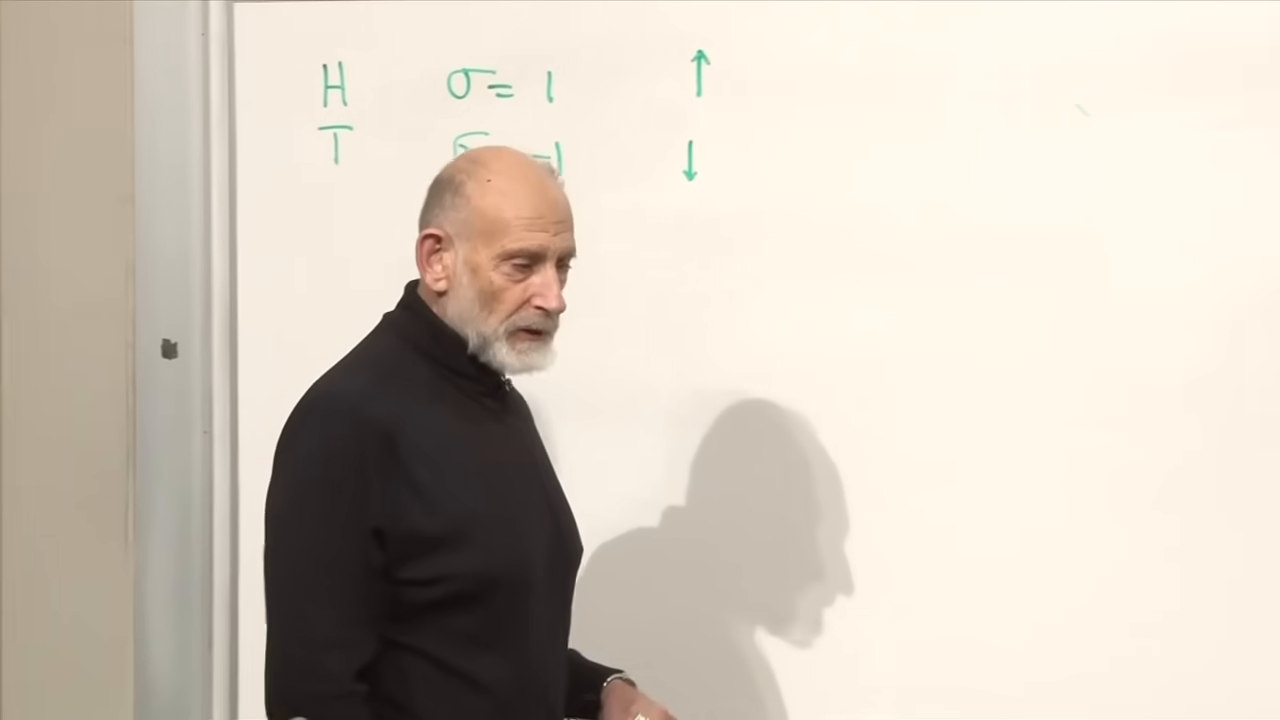
\includegraphics[width=0.78\textwidth]{lecture_01_figure_02.png}
  \caption{칠판에는 서로 동등한 표기 \(H/T\), \(\sigma=\pm1\)와 위/아래 화살표가 제시되어 있다. 여기서 화살표는 고전적 모형이 아니라 표기법으로 시작한다.}
  \lectureframe{00:22:44}
\end{figure}

\begin{classroomqa}
\audiencequestion{앞면과 뒷면은 물리계와 어떤 관계가 있나요?}
\lecturerresponse{익숙한 이름 두 개를 제공한다는 것 외에는 아무 관계도 없습니다. 큐비트는 이 측정에서 가능한 결과가 두 가지이며, 앞면과 뒷면은 그에 붙인 임시 표지입니다. \(\pm1\) 표기는 방정식에 넣을 수 있어서 선택한 것입니다.}
\end{classroomqa}

\subsection{장치를 블랙박스로 보기}

실험에는 두 번째 계인 장치 \(A\)가 필요하다. 지금은 다음 세 가지 특징을 지닌 추상적 블랙박스로 두자:
\begin{enumerate}
  \item 공간적 방향이 있으며, \emph{이 면이 위로} 오도록 표시한다;
  \item 큐비트와 상호작용할 수 있는 센서가 있다;
  \item 처음에는 비어 있고, 나중에는 \(+1\) 또는 \(-1\)를 표시하는 표시부가 있다.
\end{enumerate}
검출기의 세부 사항은 일부러 뒤로 미룬다. 좋은 검출기는 계와 기록 사이에 신뢰할 수 있는 관계를 제공하는 것으로 조작적으로 정의된다. 상호작용이 일어나는 순간에 관찰자가 지켜보고 있을 필요는 없다. 장치가 결과를 기록하고 나중에 읽을 수 있기 때문이다.

표시부에 \(+1\)가 나온다고 하자. 장치를 초기의 빈 상태로 되돌린 뒤, 독립적인 시간 변화가 일어나기 전에 같은 측정을 곧바로 반복한다. 충실한 검출기라면 다시 \(+1\)를 표시한다. 첫 결과가 \(-1\)라면, 즉시 반복해도 마찬가지로 계속 \(-1\)가 나온다:
\begin{equation}
\begin{aligned}
  +1&\longrightarrow +1\longrightarrow +1\longrightarrow\cdots,\\
  -1&\longrightarrow -1\longrightarrow -1\longrightarrow\cdots.
\end{aligned}
\end{equation}
따라서 첫 측정은 \emph{준비}로 볼 수 있다. 첫 측정은 같은 측정을 곧바로 반복하면 확정된 결과가 나오는 상태로 큐비트를 남긴다.

이 반복 가능성은 선택적인 철학적 해석이 아니다. 반복 가능성이 없다면 측정을 확인할 조작적 방법도 없다. 결함 있는 장치는 결과를 반복하지 못할 수 있지만, 그렇다면 여기서 정의하는 이상적인 측정을 수행하는 것이 아니다.

\begin{classroomqa}
\audiencequestion{이게 벌써 파동 함수의 붕괴인가요?}
\lecturerresponse{그런 표현은 나중에 도입할 수 있습니다. 지금 단계에서는 조작적 진술이면 충분합니다. 측정은 결과를 내고, 같은 측정을 곧바로 반복하면 그 결과가 재현되는 상태를 준비합니다. 과정에 이름을 붙이는 것만으로 아직 그 과정이 설명되는 것은 아닙니다.}
\end{classroomqa}

\section{방향과 고전적 지침의 실패}

똑바로 세운 장치에서 \(+1\)가 나오도록 큐비트를 준비하자. 장치를 \(180^\circ\)만큼 돌린 뒤 측정을 반복한다. 이번에는 \(-1\)가 나온다. 뒤집힌 장치로 측정을 반복하면 \(-1\)가 확인되고, 장치를 다시 똑바로 세우면 \(+1\)가 나온다.

이 결과는 방향에 따른 실제 차이를 보여준다. 위/아래 표기가 완전히 자의적인 것은 아니다. 검출기를 뒤집으면 부호도 바뀐다. 큐비트가 그저 작은 벡터이고 검출기는 자기 축 방향의 벡터 성분을 측정한다고 결론짓고 싶을 수 있다. 그러나 그런 유혹은 믿기 전에 검증해야 한다.

\begin{figure}[htbp]
  \centering
  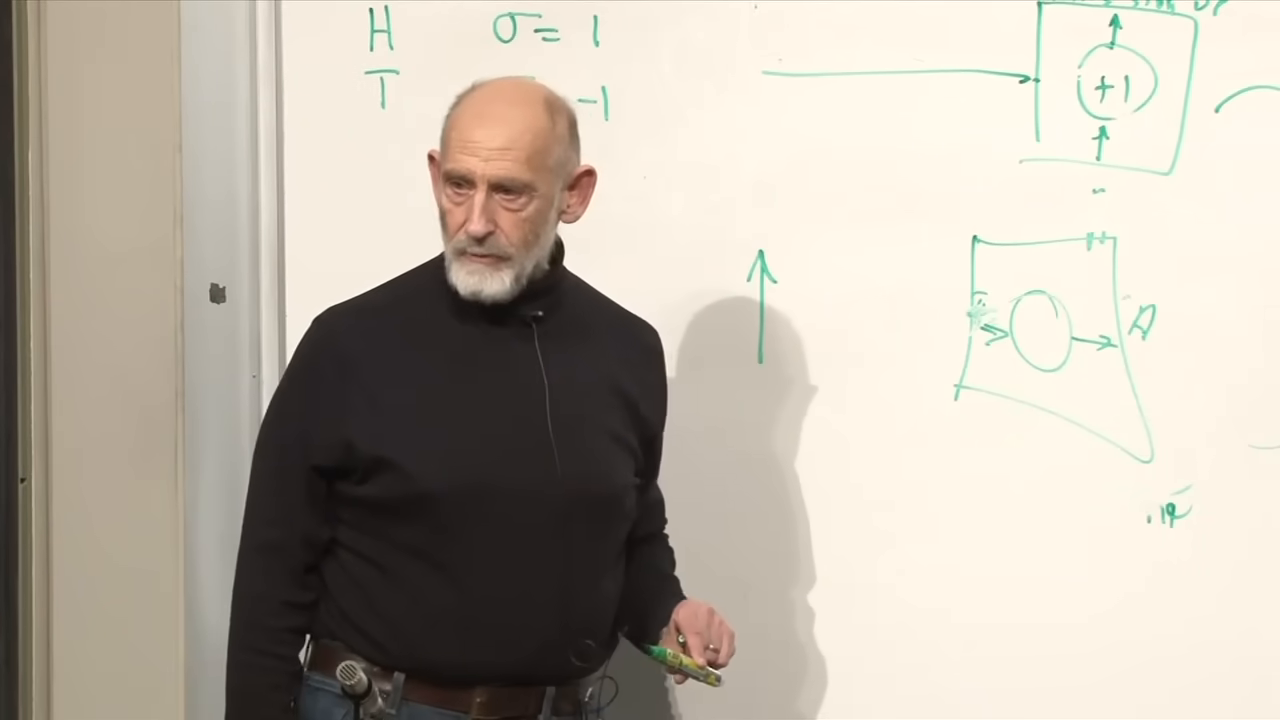
\includegraphics[width=0.82\textwidth]{lecture_01_figure_03.png}
  \caption{칠판의 위쪽 방향 준비와 서로 다른 방향의 분석기. 수업 중 분필 화살표 하나의 방향이 나중에 바로잡혔지만, 논증에서 중요한 것은 분석기의 축뿐이다.}
  \lectureframe{00:36:21}
\end{figure}

\subsection{수평 방향 측정}

검출기를 \(90^\circ\)만큼 돌린다. 준비된 큐비트가 보통의 위쪽 지침이라면 수평 검출기 축 방향 성분은 0일 것이다:
\begin{equation}
  \hat{\mathbf x}\cdot\hat{\mathbf z}=0.
\end{equation}
양자 장치는 0을 표시하지 않는다. 각각의 시행에서는 \(+1\) 또는 \(-1\)만 나온다.

\begin{figure}[htbp]
  \centering
  \resizebox{\linewidth}{!}{%
  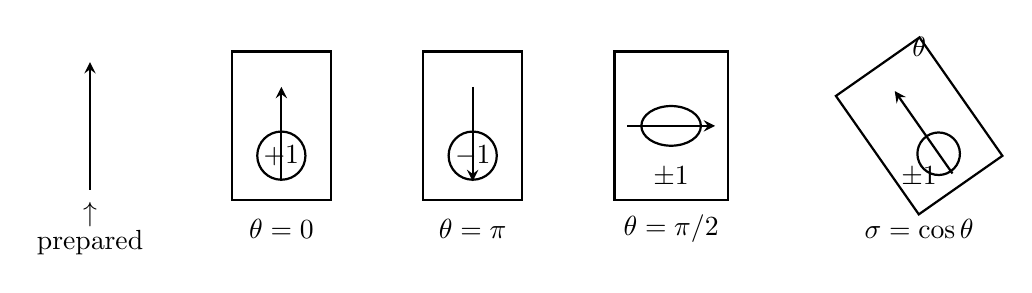
\begin{tikzpicture}[>=stealth,thick,scale=0.90]
    \draw[->] (0,0)--(0,1.8);
    \node at (0,-0.35) {\(\uparrow\)};
    \node at (0,-0.75) {prepared};

    \draw (2.0,-0.15) rectangle (3.4,1.95);
    \draw (2.7,0.48) circle (0.34);
    \draw[->] (2.7,0.12)--(2.7,1.45);
    \node at (2.7,0.48) {\(+1\)};
    \node at (2.7,-0.55) {\(\theta=0\)};

    \draw (4.7,-0.15) rectangle (6.1,1.95);
    \draw (5.4,0.48) circle (0.34);
    \draw[->] (5.4,1.45)--(5.4,0.12);
    \node at (5.4,0.48) {\(-1\)};
    \node at (5.4,-0.55) {\(\theta=\pi\)};

    \draw (7.4,-0.15) rectangle (9.0,1.95);
    \draw (8.2,0.90) ellipse (0.42 and 0.28);
    \draw[->] (7.58,0.90)--(8.82,0.90);
    \node at (8.2,0.18) {\(\pm1\)};
    \node at (8.2,-0.55) {\(\theta=\pi/2\)};

    \begin{scope}[shift={(11.7,0.90)},rotate=35]
      \draw (-0.72,-1.02) rectangle (0.72,1.02);
      \draw (0,-0.48) circle (0.30);
      \draw[->] (0,-0.82)--(0,0.60);
    \end{scope}
    \node at (11.7,0.18) {\(\pm1\)};
    \node at (11.7,-0.55) {\(\expect{\sigma}=\cos\theta\)};
    \node at (11.7,2.02) {\(\theta\)};
  \end{tikzpicture}
  }%
  \caption{분석기 배열을 재구성한 그림. 회전하면 통계는 달라지지만 개별 결과의 집합은 달라지지 않는다.}
\end{figure}

똑바로 세운 장치로 큐비트를 많이 준비하고, 결과가 \(+1\)인 큐비트만 남긴다. 남은 큐비트를 각각 수평 장치로 한 번씩 측정한다. 시행의 절반에서는 \(+1\)가, 나머지 절반에서는 \(-1\)가 나오며, 앙상블 평균은 0이다:
\begin{equation}
  \expect{\sigma}_{\pi/2}=0.
\end{equation}
평균은 고전적 지침의 사라지는 수평 성분과 비슷하지만, 개별 기록은 그렇지 않다. 고전적 값 \(0\)은 두 이산적 결과 사이의 통계적 균형으로 대체되었다.

\begin{classroomqa}
\audiencequestion{수평 측정 뒤에 버리지 않고 같은 큐비트를 계속 두면 어떻게 되나요?}
\lecturerresponse{첫 수평 측정 결과가 \(+1\)라고 하자. 같은 큐비트에 수평 측정을 반복하면 매번 다시 \(+1\)가 나온다. 첫 수평 측정은 수평축을 기준으로 그 큐비트를 준비한 것이다. 반반의 통계를 얻으려면 한 결과를 반복해서 확인하는 대신, 여러 큐비트로 준비와 측정의 전체 실험을 반복해야 한다.}
\end{classroomqa}

\subsection{양립할 수 없는 준비}

축을 어떤 순서로 사용하는지가 중요하다. \(+1\)로 준비한 뒤 수평 방향으로 측정한다. 첫 수평 측정 결과는 무작위다. 수평 결과가 한 번 나오고 나면, 수평 측정을 곧바로 반복했을 때는 확정된 결과가 나온다. 이제 검출기를 다시 수직축으로 돌린다. 수직 측정 결과는 다시 무작위가 된다.

\(M_z\)와 \(M_x\)가 두 축 방향의 측정을 나타낸다고 할 때, 기호로 쓰면 다음과 같다:
\begin{equation}
\begin{aligned}
  M_z&:+1,\\
  M_x&:\pm1,\\
  M_x&:\text{same result},\\
  M_z&:\pm1.
\end{aligned}
\end{equation}
중간의 \(x\)-측정은 원래의 수직 상태를 보존한 채 수평 성분만 알아낸 것이 아니다. 새로운 상태를 준비했으며, 원래의 수직 방향 확정성은 사라졌다.

\begin{classroomqa}
\audiencequestion{검출기는 첫 번째 답을 기억하나요? 같은 큐비트가 다시 왔는지 새 큐비트가 왔는지 어떻게 알 수 있나요?}
\lecturerresponse{반복 가능성은 검출기가 숨겨진 기억을 대조해서 얻는 성질이 아니라 측정된 큐비트의 성질입니다. 측정 뒤 큐비트는 같은 측정을 곧바로 반복하면 같은 답을 내는 상태에 있습니다. 다르게 준비한 큐비트를 제시하면 결과는 그 준비 상태에 따라 달라집니다. 어떤 물리계를 측정하고 있는지 추적하는 것은 실험실에서 하는 통상적인 기록 관리입니다.}
\end{classroomqa}

\begin{classroomqa}
\audiencequestion{그러니까 관측 행위가 해당 큐비트를 준비하는 건가요?}
\lecturerresponse{그렇습니다. 측정으로 큐비트가 준비되고 나면, 다른 시간 변화나 양립할 수 없는 측정이 개입할 때까지 같은 측정에서 같은 답이 나옵니다.}
\end{classroomqa}

\section{임의의 각도로 회전한 분석기}

검출기 축이 앙상블을 준비한 축과 \(\theta\)만큼 이루는 각도를 둔다. 각 시행에서 여전히 다음 결과 중 하나가 나온다:
\begin{equation}
  \sigma=\pm1.
\end{equation}
상대도수는 각도에 따라 달라지며 평균은 다음과 같다:
\begin{equation}
  \expect{\sigma}_{\theta}=\cos\theta.
  \label{eq:qml1-cosine-mean}
\end{equation}
극한 경우는 다음과 같다:
\begin{align}
  \expect{\sigma}_{0}&=+1,\\
  \expect{\sigma}_{\pi/2}&=0,\\
  \expect{\sigma}_{\pi}&=-1.
\end{align}
\(\theta=0\) 부근에서는 대부분 \(+1\)가 나오고, 간혹 \(-1\)가 나온다. \(\theta=\pi\) 부근에서는 대부분 \(-1\)가 나오고, 간혹 \(+1\)가 나온다.

\begin{figure}[htbp]
  \centering
  \includegraphics[width=0.82\textwidth]{lecture_01_figure_04.png}
  \caption{임의의 각도 실험에서 실제로 사용한 칠판 그림. 수직 방향으로 준비된 앙상블이 \(\theta\)만큼 기울어진 분석기로 들어간다.}
  \lectureframe{00:48:55}
\end{figure}

벡터처럼 부드럽게 변하는 양은 개별 결과가 아니라 앙상블 평균이다. \(p_+(\theta)\)와 \(p_-(\theta)\)가 두 결과의 확률이라면,
\begin{equation}
  p_+ + p_-=1,
  \qquad
  p_+-p_-=\cos\theta.
\end{equation}
따라서,
\begin{equation}
\begin{aligned}
  p_+(\theta)&=\frac{1+\cos\theta}{2}
  =\cos^2\frac{\theta}{2},\\
  p_-(\theta)&=\frac{1-\cos\theta}{2}
  =\sin^2\frac{\theta}{2}.
\end{aligned}
  \label{eq:qml1-half-angle-probabilities}
\end{equation}
\editorialnote{강의에서는 두 결과와 그 평균 \(\cos\theta\)을 제시한다. 식~\eqref{eq:qml1-half-angle-probabilities}은 그 진술들에서 바로 따라오는 대수적 결과이며, 암시된 빈도 법칙을 명시적으로 나타낸다.}

\begin{classroomqa}
\audiencequestion{준비되지 않은 큐비트 앙상블에서도 평균이 \(\cos\theta\)인가요?}
\lecturerresponse{편극되지 않은 앙상블에서는 특정 방향이 선택되지 않으므로 평균은 0입니다. \(\theta\) 의존성은 먼저 명확한 축을 따라 준비한 앙상블을 가리킵니다.}
\end{classroomqa}

\begin{classroomqa}
\audiencequestion{큐비트에 중간 동역학이 없다면 왜 앙상블 전체가 필요한가요?}
\lecturerresponse{한 큐비트에 처음 기울어진 측정을 하면 표본 하나를 얻습니다. 같은 큐비트에서 곧바로 측정을 반복하면 그 표본을 확인할 뿐입니다. 독립적인 시행을 하려면 동일하게 준비된 큐비트마다 기울어진 분석기로 한 번씩 측정해야 합니다.}
\end{classroomqa}

\begin{classroomqa}
\audiencequestion{플러스와 마이너스가 이어지는 순서에 규칙성이나 고차 상관관계가 있나요?}
\lecturerresponse{이 실험에서는 각 시행을 서로 독립이고 상관관계가 없는 것으로 간주합니다. 한 번의 시행에서 각 결과가 나올 확률은 \(\theta\)에 따라 달라지지만, 그 밖의 순서 패턴을 주장하는 것은 아닙니다.}
\end{classroomqa}

\subsection{이상화한 부분}

현재로서는 장치를 방향을 연속적으로 조절할 수 있고 판독값은 이산적인 고전적 물체로 취급한다. \emph{계}와 \emph{검출기}의 구분은 잠정적이다. 검출기도 물리계이므로 결국 양자역학을 따라야 한다. 완전한 설명에서는 계와 장치를 함께 다루겠지만, 그러려면 아직 배우지 않은 수학적 도구가 필요하다.

\begin{classroomqa}
\audiencequestion{검출기도 또 다른 두 상태 계일 뿐인가요?}
\lecturerresponse{검출기에도 물리적 상태가 있으며, 궁극적으로 양자적 기술에 포함되어야 합니다. 지금은 조작적인 구분을 유지합니다. 큐비트는 양자역학으로 기술하는 대상이고, 방향이 정해진 검출기는 안정적인 고전적 기록을 제공합니다. 나중에는 결합된 계를 서로 상호작용하는 양자계로 분석해야 합니다.}
\end{classroomqa}

\begin{classroomqa}
\audiencequestion{검출기를 돌리는 축을 바꾸면 여기 나온 단일 각도보다 더 많은 구조가 생기나요?}
\lecturerresponse{그렇습니다. 3차원 전체를 다루는 이야기는 더 풍부합니다. 한 평면에서의 회전은 그중 가장 단순한 단면이며, 앞으로 다룰 더 완전한 설명과 모순되지 않습니다.}
\end{classroomqa}

\begin{classroomqa}
\audiencequestion{검출기가 \(-1\)와 \(+1\) 사이의 연속적인 값을 낼 수 있나요?}
\lecturerresponse{방향은 연속적으로 변하지만, 이상적인 큐비트 판독값은 항상 \(+1\) 또는 \(-1\)입니다. 연속성은 개별 결과가 아니라 방향이 변할 때 확률과 평균에 나타납니다.}
\end{classroomqa}

\section{지침과 추상적 벡터}

이제 실험적 사실은 잠시 제쳐 두고 수학을 살펴보자. 물리적 공간의 보통 화살표를 \emph{지침}이라 부르겠다. 수학적 벡터는 더 일반적인 개념이다. 벡터 공간의 원소이며, 일상 공간의 어떤 방향을 가리킬 필요는 없다.

\begin{definition}
복소 벡터 공간 \(V\)은 벡터의 덧셈과 복소 스칼라에 의한 곱셈이 정의되어 있고, 통상적인 선형성 규칙을 만족하는 벡터들의 집합이다. 특히 \(u,v,w\in V\)와 \(a,b\in\mathbb C\)에 대해,
\begin{align}
  u+v&=v+u,\\
  (u+v)+w&=u+(v+w),\\
  a(u+v)&=au+av,\\
  (a+b)u&=au+bu,\\
  (ab)u&=a(bu),\\
  1u&=u.
\end{align}
영벡터 \(0\)가 있으며 모든 \(u\)에 대해 덧셈 역원 \(-u\)가 존재한다.
\end{definition}

칠판 논의에서는 처음에 연산과 닫힘성만 강조한다:
\begin{equation}
\begin{aligned}
  u,v\in V&\Longrightarrow u+v\in V,\\
  a\in\mathbb C,\ u\in V&\Longrightarrow au\in V.
\end{aligned}
\end{equation}
질문에 답하면서 영벡터와 교환 법칙도 덧붙인다. 나머지 익숙한 공리들은 구체적인 열벡터 모형을 도입할 때 이미 사용하는 성질을 명시적으로 적은 것이다.

실수는 \(\mathbb R\) 위의 1차원 벡터 공간을 이룬다. 복소수는 \(\mathbb C\) 위의 1차원 벡터 공간이자 \(\mathbb R\) 위의 2차원 벡터 공간을 이룬다. 복소수 값을 갖는 함수 \(\psi(x)\) 역시 다음 성질 때문에 복소 벡터 공간을 이룬다:
\begin{equation}
  (\psi+\phi)(x)=\psi(x)+\phi(x),
  \qquad
  (z\psi)(x)=z\psi(x).
\end{equation}
이 함수 공간의 예는 나중에 중심적인 역할을 하겠지만, 먼저 유한한 열벡터로 구조를 살펴보면 더 이해하기 쉽다.

\begin{classroomqa}
\audiencequestion{벡터와 벡터 공간은 어떻게 다른가요?}
\lecturerresponse{벡터는 원소 하나를 가리킵니다. 벡터 공간은 그런 원소 전체와, 그 원소들을 더하고 스칼라배하는 규칙을 함께 가리킵니다. 하나의 수가 단일 대상이고 수 체계가 연산을 갖춘 원소들의 모임인 것과 같습니다.}
\end{classroomqa}

\section{두 성분 복소 열벡터}

추상적인 벡터를 디랙 표기법으로 \(\ket{\alpha}\)라 쓰자. 구체적인 표현은 다음과 같다:
\begin{equation}
  \ket{\alpha}
  \longleftrightarrow
  \begin{pmatrix}
    \alpha_1\\
    \alpha_2
  \end{pmatrix},
  \qquad
  \alpha_1,\alpha_2\in\mathbb C.
\end{equation}
다음과 같이 두면,
\begin{equation}
  \ket{\beta}
  \longleftrightarrow
  \begin{pmatrix}
    \beta_1\\
    \beta_2
  \end{pmatrix},
\end{equation}
덧셈과 스칼라배는 각 성분별로 정의된다:
\begin{align}
  \ket{\alpha}+\ket{\beta}
  &\longleftrightarrow
  \begin{pmatrix}
    \alpha_1+\beta_1\\
    \alpha_2+\beta_2
  \end{pmatrix},\\
  z\ket{\alpha}
  &\longleftrightarrow
  \begin{pmatrix}
    z\alpha_1\\
    z\alpha_2
  \end{pmatrix},
  \qquad z\in\mathbb C.
\end{align}

\begin{figure}[htbp]
  \centering
  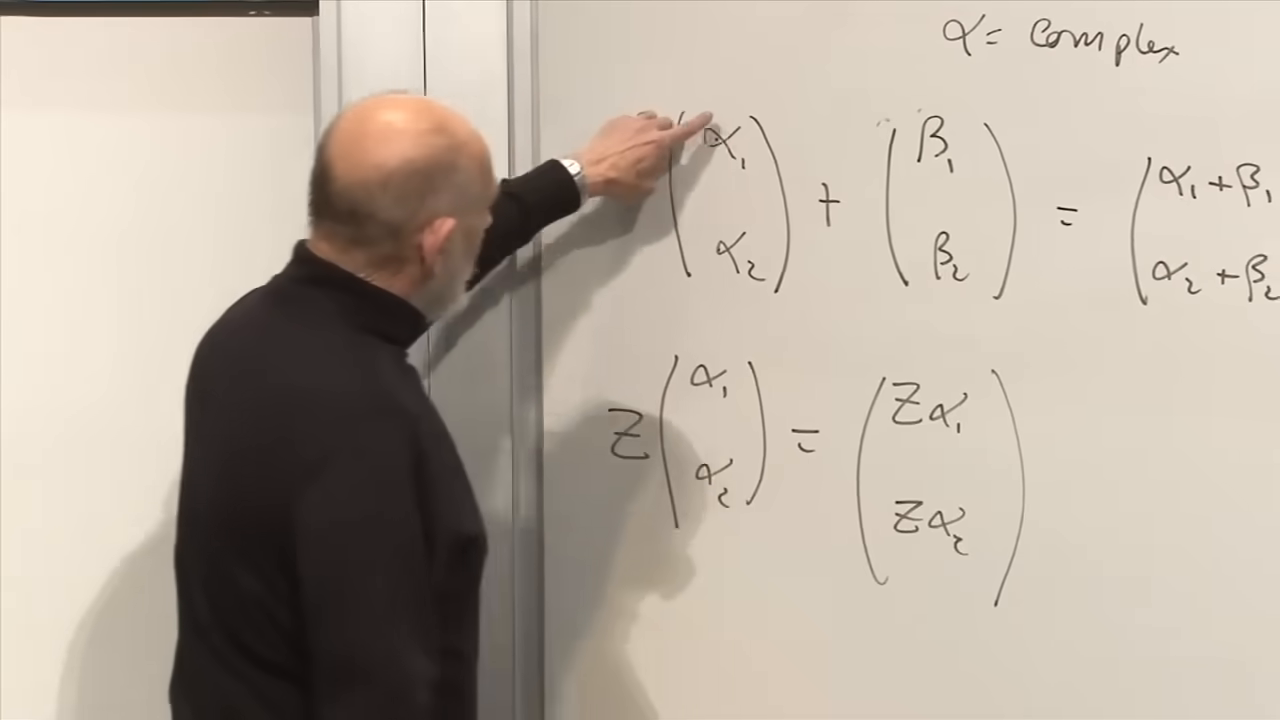
\includegraphics[width=0.88\textwidth]{lecture_01_figure_05.png}
  \caption{복소 열벡터 둘의 덧셈과 열벡터에 복소 스칼라를 곱하는 성분별 규칙.}
  \lectureframe{01:14:28}
\end{figure}

영벡터는 다음과 같다:
\begin{equation}
  \ket{0}
  =
  \begin{pmatrix}
    0\\
    0
  \end{pmatrix},
  \qquad
  \ket{\alpha}+\ket{0}=\ket{\alpha}.
\end{equation}
길이가 3인 열벡터도 또 하나의 벡터 공간을 이루며, 고정된 임의의 길이에 대해서도 마찬가지다. 두 열벡터는 서로 다른 공간에 속하고 두 공간을 연결하는 성분별 규칙이 없으므로, 성분이 2개인 열벡터와 성분이 3개인 열벡터는 더할 수 없다.

\begin{classroomqa}
\audiencequestion{열벡터는 행렬인가요?}
\lecturerresponse{일반적인 용어로는 열이 하나인 행렬입니다. 이 강의에서는 \emph{행렬}이라는 말을 보통 정사각 배열에 사용하고, 열이 하나인 배열은 열벡터라고 부릅니다. 이는 용어상의 구분일 뿐 대수에 대한 견해 차이가 아닙니다.}
\end{classroomqa}

\begin{classroomqa}
\audiencequestion{벡터 덧셈은 순서에 따라 달라지나요?}
\lecturerresponse{아니요. 성분별 덧셈은 복소수의 교환 법칙을 그대로 따른다:
\[
  \ket{\alpha}+\ket{\beta}
  =
  \ket{\beta}+\ket{\alpha}.
\]
이것은 벡터 공간의 공리 가운데 하나다.}
\end{classroomqa}

\section{쌍대벡터: 브라와 켓}

모든 켓 \(\ket{A}\)에는 쌍대 공간의 대응 벡터가 있으며, \(\bra{A}\)로 쓴다. 켓에서 브라로 가는 사상은 덧셈에 대해서는 선형이고 복소 스칼라는 켤레 복소수로 바꾼다:
\begin{align}
  \ket{A}+\ket{B}
  &\longleftrightarrow
  \bra{A}+\bra{B},\\
  z\ket{A}
  &\longleftrightarrow
  z^*\bra{A}.
  \label{eq:qml1-antilinear-dual}
\end{align}
두 번째 규칙이 복소수의 핵심적인 특징이다. 스칼라배한 켓의 쌍대벡터에는 스칼라의 복소켤레를 곱한다.

\begin{figure}[htbp]
  \centering
  \includegraphics[width=0.86\textwidth]{lecture_01_figure_06.png}
  \caption{켓과 브라의 대응 및 두 가지 규칙. 합은 합으로 대응하고, 스칼라배에서는 복소켤레를 취한다.}
  \lectureframe{01:23:15}
\end{figure}

두 성분 표현에서는,
\begin{equation}
  \ket{\alpha}
  =
  \begin{pmatrix}
    \alpha_1\\
    \alpha_2
  \end{pmatrix}
  \qquad\Longrightarrow\qquad
  \bra{\alpha}
  =
  \begin{pmatrix}
    \alpha_1^*&\alpha_2^*
  \end{pmatrix}.
  \label{eq:qml1-bra-from-ket}
\end{equation}
복소켤레가 쌍대 대응을 구현하고, 행 표기는 두 종류의 대상을 눈에 띄게 구별해 준다. 식~\eqref{eq:qml1-bra-from-ket}은 식~\eqref{eq:qml1-antilinear-dual}도 직접 확인해 준다.

\section{내적}

\(\ket{\alpha}\)와 \(\ket{\beta}\)가 주어졌을 때, \(\beta\)에 대응하는 브라와 \(\alpha\) 켓을 결합하면 다음과 같다:
\begin{equation}
  \braket{\beta}{\alpha}
  =
  \begin{pmatrix}
    \beta_1^*&\beta_2^*
  \end{pmatrix}
  \begin{pmatrix}
    \alpha_1\\
    \alpha_2
  \end{pmatrix}
  =
  \beta_1^*\alpha_1+\beta_2^*\alpha_2.
  \label{eq:qml1-inner-product}
\end{equation}
\emph{브래킷}이라는 말은 \emph{브라}와 \emph{켓}을 결합해 만든 이름이다. 이는 내적의 복소수 유사체다. 대응하는 성분끼리 곱해 더하되 브라 쪽에는 복소켤레를 취한다.

\begin{figure}[htbp]
  \centering
  \includegraphics[width=0.88\textwidth]{lecture_01_figure_07.png}
  \caption{칠판에서 내적 \(\braket{\beta}{\alpha}\)을 계산하면 \(\beta_1^*\alpha_1+\beta_2^*\alpha_2\)이 된다.}
  \lectureframe{01:31:25}
\end{figure}

벡터의 순서를 바꾸면 다음과 같다:
\begin{equation}
  \braket{\alpha}{\beta}
  =
  \alpha_1^*\beta_1+\alpha_2^*\beta_2
  =
  \braket{\beta}{\alpha}^{*}.
  \label{eq:qml1-conjugate-symmetry}
\end{equation}
따라서 일반적으로 순서에 따라 값이 달라지지만, 달라지는 것은 복소켤레뿐이다.

\begin{classroomqa}
\audiencequestion{한쪽에 복소켤레를 취하지 않고 복소 벡터의 곱을 정의할 수 있나요?}
\lecturerresponse{그런 쌍선형 표현을 만들 수는 있지만, 벡터를 자기 자신과 곱한 결과가 실수이거나 양수일 필요가 없게 됩니다. 양자역학에 유용한 구조는 그것이 아닙니다. 켤레를 취하는 에르미트 내적은 앞으로 필요한 노름과 확률 구조를 제공한다.}
\end{classroomqa}

\subsection{노름과 양성}

식~\eqref{eq:qml1-inner-product}에서 \(\beta=\alpha\)로 두면,
\begin{equation}
  \braket{\alpha}{\alpha}
  =
  \alpha_1^*\alpha_1+\alpha_2^*\alpha_2
  =
  |\alpha_1|^2+|\alpha_2|^2.
  \label{eq:qml1-norm-square}
\end{equation}
이 값은 자기 자신의 복소켤레와 같으므로 실수다. 이 값은 음이 아니며, 영벡터일 때에만 0이 된다. 길이는 다음과 같이 정의한다:
\begin{equation}
  \|\alpha\|
  =
  \sqrt{\braket{\alpha}{\alpha}}.
\end{equation}
따라서 복소 성분으로도 통상적인 음이 아닌 실수 길이를 얻는다.

\begin{figure}[htbp]
  \centering
  \includegraphics[width=0.88\textwidth]{lecture_01_figure_08.png}
  \caption{자기 자신과의 내적을 칠판에서 계산하면 \(\braket{\alpha}{\alpha}=|\alpha_1|^2+|\alpha_2|^2\), 즉 노름의 제곱이 된다.}
  \lectureframe{01:34:40}
\end{figure}

\section{직교성과 차원}

두 벡터의 내적이 영이면 서로 직교한다:
\begin{equation}
  \braket{\beta}{\alpha}=0.
  \label{eq:qml1-orthogonality}
\end{equation}
켤레 대칭성에 따라 이 관계는 순서와 무관하다:
\begin{equation}
  \braket{\beta}{\alpha}=0
  \quad\Longrightarrow\quad
  \braket{\alpha}{\beta}
  =
  \braket{\beta}{\alpha}^{*}
  =0.
\end{equation}

두 성분 공간에서 가장 간단한 직교 쌍은 다음과 같다:
\begin{equation}
  \ket{e_1}
  =
  \begin{pmatrix}
    1\\
    0
  \end{pmatrix},
  \qquad
  \ket{e_2}
  =
  \begin{pmatrix}
    0\\
    1
  \end{pmatrix},
  \qquad
  \braket{e_1}{e_2}=0.
  \label{eq:qml1-standard-basis}
\end{equation}

\begin{figure}[htbp]
  \centering
  \includegraphics[width=0.88\textwidth]{lecture_01_figure_09.png}
  \caption{칠판에서 표준 직교 열벡터 \((1,0)^{\mathsf T}\)와 \((0,1)^{\mathsf T}\)를 구성한다.}
  \lectureframe{01:39:50}
\end{figure}

차원은 서로 직교하는 영이 아닌 벡터의 최대 개수로 특징지을 수 있다. 이차원 공간에는 그런 벡터가 두 개 있을 수 있지만 세 번째 벡터는 있을 수 없다. 이를 구체적으로 살펴보기 위해 다음과 같이 두자:
\begin{equation}
  \ket{v}
  =
  \begin{pmatrix}
    v_1\\
    v_2
  \end{pmatrix}
\end{equation}
이 벡터가 ~\eqref{eq:qml1-standard-basis}에 나오는 두 벡터 모두와 직교한다고 하자. 그러면
\begin{equation}
  \braket{e_1}{v}=v_1=0,
  \qquad
  \braket{e_2}{v}=v_2=0,
\end{equation}
따라서 \(\ket{v}=\ket{0}\)이다. 두 벡터 모두와 직교하는 세 번째 영이 아닌 벡터는 존재하지 않는다.

\begin{classroomqa}
\audiencequestion{영벡터는 모든 벡터와 직교하니 하나를 더 셀 수 있지 않나요?}
\lecturerresponse{그렇습니다. 그래서 정의에 서로 직교하는 \emph{0이 아닌} 벡터라고 명시해야 합니다. 영벡터는 독립적인 방향을 나타내지 않으므로 차원을 셀 때 제외한다.}
\end{classroomqa}

\begin{remark}
열벡터 표현에서 차원은 성분의 개수와 같다. 직교성의 정의는 더 추상적이며, 좌표를 이미 선택했는지에 의존하지 않는다.
\end{remark}

\section{칠판에서 이어진 질문}

\begin{classroomqa}
\audiencequestion{같은 구조를 함수 벡터 공간에도 적용할 수 있나요?}
\lecturerresponse{그렇습니다. 함수는 연속적으로 색인된 성분들 \(\psi(x)\)을 갖는 열벡터로 볼 수 있습니다. 덧셈과 스칼라배는 점별로 합니다. 이에 대응하는 내적은 유한합이 아니라 적분이 되며, 그 구성은 나중에 다룹니다.}
\end{classroomqa}

\begin{classroomqa}
\audiencequestion{켓에 브라를 곱하면 행렬이 되나요?}
\lecturerresponse{그렇습니다. 내적 \(\bra{\beta}\ket{\alpha}\)은 행과 열을 축약해 수 하나를 만듭니다. 순서를 반대로 한 \(\ket{\alpha}\bra{\beta}\)은 외적이 되어 정사각 행렬을 만듭니다. 내적과 외적은 모두 중요해진다.}
\end{classroomqa}

\begin{classroomqa}
\audiencequestion{측정은 큐비트에 영향을 주나요, 아니면 단지 그 상태를 드러내나요?}
\lecturerresponse{영향을 줍니다. 새로운 축 방향의 첫 측정은 새로운 상태를 준비합니다. 그래서 그 측정을 반복하면 결과가 확인되지만, 이전 축으로 돌아가면 불확실성이 다시 나타납니다. 피할 수 없는 이 교란은 원칙적으로 임의로 약하게 할 수 있는 이상화된 고전적 측정과 양자 실험을 구별합니다.}
\end{classroomqa}

\section{구성의 두 부분}

이제 아직 서로 연결되지 않은 두 부분을 살펴보았다. 실험 부분의 내용은 다음과 같다:
\begin{enumerate}
  \item 이상적인 큐비트 측정의 결과는 \(\pm1\)뿐이다;
  \item 같은 측정을 곧바로 반복하면 결과가 확인된다;
  \item 검출기 축을 바꾸면 측정으로 준비되는 상태도 달라진다;
  \item 준비된 앙상블에서 분석기를 \(\theta\)만큼 기울이면 평균은 \(\cos\theta\)이다.
\end{enumerate}
수학 부분의 내용은 다음과 같다:
\begin{enumerate}
  \item 양자 상태는 고전적 점이 아니라 벡터로 표현한다;
  \item 관련 벡터들은 복소 벡터 공간을 이룬다;
  \item 켓에는 쌍대 브라가 대응하며, 복소수 스칼라배에 대해 브라는 반선형으로 변환된다;
  \item 에르미트 내적은 길이, 직교성, 차원을 정의한다.
\end{enumerate}

이제 다음 과제는 이 두 부분을 연결하는 것이다. 큐비트의 2차원 복소 상태 공간은 분석기 실험의 반복성, 무작위성, 그리고 각도에 따른 통계를 재현해야 한다. 숨겨진 고전적 그림이 아니라 바로 이 연결에서 양자역학이 시작된다.
